\section{Optical Dipole Trapping}

The use of \glspl{odt} in the cold-atom electron source will allow greater stability of the atom cloud during ionisation and extraction as well as increasing the density of the atom cloud during these phases with corresponding increases in density.

\subsection{History of optical dipole trapping}
The use of the optical dipole force as a confining mechanism was first proposed by Askar'yan in 1962\cite{askaryan_effects_1962} for plasmas and neutral atoms. Ashkin successfully demonstrated the trapping of micron-size latex spheres suspended in water using a focused Gaussian lasers in 1970\cite{ashkin_acceleration_1970}. The first optical trapping of atoms was demonstrated by Chu et. al. in 1986\cite{chu_experimental_1986} where a \gls{odt} was used to trap sodium atoms.

\subsection{Theory of Dipole Trapping}
\Glspl{odt} are sometimes considered to be the simplest form of atom trap since then consit solely of a focused, Gaussian laser beam detuned from the atomic resonances.

\subsubsection{Trapping potential}
The intensity of a Gaussian laser beam at the beam waist varies with $r$ as
\begin{equation}
I(r) = I_0e^{-r^2 / w_0^2},
\end{equation}
where $I_0$ is the intensity at the centre of the beam at the waist, $r$ is the radial distance from the centre of beam and $w_0$ is the beam radius at the focus.

The ground state light shift is given by\cite{metcalf_laser_1999}
\begin{equation}
\Delta E_g = \frac{\hbar \Omega^2}{4\delta},
\end{equation}
where the Rabi frequency $\Omega^2= \gamma^2 I / 2 I_s$ and $\gamma$ is the linewidth, $I$ is the light intensity and $I_s$ is the saturation intensity. Thus the light shift is larger at points of high intensity such as the centre of the beam and the beam focus.

In order to trap the laser is detuned below the resonances such that $\delta = \omega_l - \omega_a < 0$ where $\omega_l$ is the laser frequency and $\omega_a$ is the atomic resonance frequency. With negative detuning the ground-state light shift is negative everywhere and thus atoms feel a force towards the centre given by the gradient of the light shift, and for $\delta \gg \Omega$ and $\delta \gg \gamma$ the force is given by
\begin{equation}
F \simeq - \frac{\hbar}{4\delta} \nabla(\Omega(r)^2) = -\frac{\hbar \gamma^2}{8\delta I_s} \nabla I (r).
\end{equation}

At the focus of a Gaussian beam this force is
\begin{equation}
F \simeq \frac{\hbar \gamma^2}{4 \delta} \frac{I_0}{I_s} \frac{r}{w_0^2} e^{-r^2/w_0^2},
\end{equation}
and thus the transverse trapping potential is given by
\begin{equation}
U = -\int dr F \simeq \frac{\hbar \gamma^2}{8\delta} \frac{I_0}{I_s} e^{-r^2/w_0^2}.
\end{equation}

It is easy to see with this equation how a negative (red) detuning will result in an inwards, trapping force and a positive (blue) detuning will result in a outwards, repulsive force. Blue detuned lasers can be used for trapping if the beam has a low intensity centre however \cite{davidson_long_1995, lee_raman_1996, ozeri_long_1999, friedman_compression_2000}.

\subsubsection{Scattering rates}
More general expressions for the trapping potential can be used to compare the potential to the scattering rate due to photon absorption \cite{grimm_optical_2000}
\begin{equation}
U_{dip}(\vec{r})=\frac{3\pi c^2}{2\omega_0^3} \frac{\gamma}{\delta} I(\vec{r})
\end{equation}
\begin{equation}
\Gamma_{sc}(\vec{r})=\frac{3\pi c^2}{2\hbar \omega_0^3}\left(\frac{\gamma}{\delta}\right)^2 I(\vec{r})
\end{equation}

The scattering rate should be kept to a minimum in order to prevent the heating atoms in the trap. Fortunately the relationships are such that for large detunings $U_{dip}\gg\Gamma_{sc}$. Such far detuned lasers however do create shallower traps and thus require more powerful lasers to create similar trap depths.

\subsection{Using an optical dipole trap in a cold-atom electron source}
An \gls{odt} can serve several purposes in the cold-atom electron source including increasing the brightness and coherence of the electron bunches as described earlier.

A number of design choices in the development of this dipole trap are under consideration such as the wavelength of the trap, the configuration of the trapping beam/s and the size of the beam waist.

\subsubsection{Available equipment}
Two main options are available as far as light sources for the trap,
\begin{itemize}
    \item a 20mW, 780nm diode laser amplified by a tapered amplifier to 1.8W,
    \item a 20W, 1064nm fibre laser.
\end{itemize}

The 780nm diode laser that seeds the tapered amplifier can be tuned away from the 780nm resonance [HOW FAR EXACTLY? what does this do to the TA?] up to [SOME NUMBER] nm. The 1064nm laser is extremely far away from the resonances which will result in reduced scattering rates however lasers with power as high as 20W require more caution in there use as well as suitable high-power optics.

\subsubsection{1064nm optical dipole traps}
\Glspl{odt} with a wavelength near 1064nm are frequently used when rubidium \glspl{bec} are being formed \cite{chikkatur_continuous_2002, couvert_quasi-monomode_2008, kleine_buning_slow_2010, lin_rapid_2009, arnold_all-optical_2011, fu_bose-einstein_2011}. These \glspl{bec} are used for many different applications including the creation of atom-lasers \cite{kleine_buning_slow_2010, chikkatur_continuous_2002, couvert_quasi-monomode_2008}, atomic clocks\cite{kleine_buning_extended_2011} and obviously further studies into \glspl{bec} themselves and related trapping mechanisms \cite{arnold_all-optical_2011, fu_bose-einstein_2011, lin_rapid_2009}.

\glspl{odt} with wavelengths at 1064nm are not only used in rubidium \glspl{bec}. They have to used to form \glspl{bec} of caesium\cite{hung_accelerating_2008}, chromium\cite{beaufils_all-optical_2008}, double-species \glspl{bec}\cite{thalhammer_double_2008}, and even molecular \glspl{bec}\cite{zwierlein_observation_2003}.

\subsubsection{``Near" 780nm optical dipole traps}
Traps made from lasers ``near'' 780nm are more often used when studying and developing trapping methods [possibly due to reduced costs?]. Such traps have detunings that vary from 0.5nm\cite{miller_rf-induced_2002} to over 60nm\cite{miller_far-off-resonance_1993, weber_analysis_2006} and are usually referred to as \glspl{fort}. Some of the things that these laser have been used to study are dipole trap loading\cite{kuppens_loading_2000}, trapping single atoms\cite{weber_analysis_2006} and the combination of an \gls{odt} with Sisyphus cooling\cite{miller_rf-induced_2002}.

\subsubsection{Configurations}
The simplest \gls{odt} consists simply of a focussed Gaussian beam\cite{chu_experimental_1986} and many of the references use this simple configuration.

\begin{figure}[h]
	\centering
	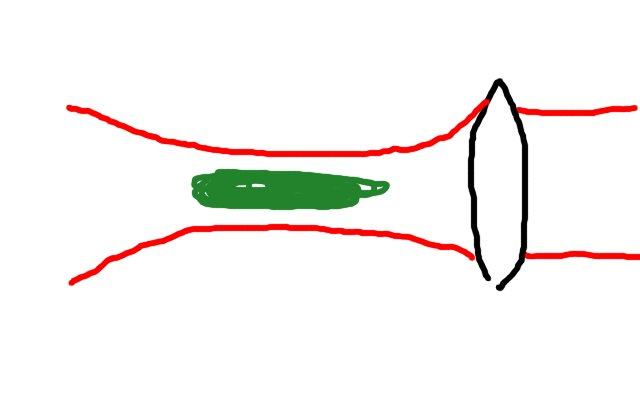
\includegraphics[scale=0.32]{figs/simpledipoletrap.jpg}
	\caption[Title]{A simple \gls{odt} configuration}
	\label{figs/MOT.pdf}
\end{figure}

Crossed dipole traps\cite{barrett_all-optical_2001, xiong_evaporative_2010, arnold_all-optical_2011, fu_bose-einstein_2011} are a more complicated configuration that can provide a stronger trap as well as control over the shape of the trap and the trapping potentials in various directions. [Examples] Unlike simple dipole traps which create long cigar-shaped traps crossed dipole traps can create spherical traps.

\begin{figure}[h]
	\centering
	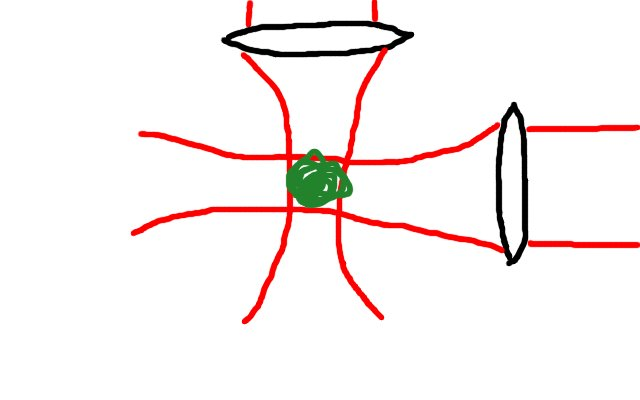
\includegraphics[scale=0.32]{figs/crosseddipoletrap.jpg}
	\caption[Title]{A crossed \gls{odt} configuration}
	\label{figs/MOT.pdf}
\end{figure}

Something about the angles involved. [refind the reference]

Crossed dipole traps do not require the beams to be at right angles. Couvert et al. \cite{couvert_quasi-monomode_2008} have their beams at 45 degrees when generating atom lasers and ANOTHER EXAMPLE.

Not trapping at the focus. [refind the reference]

\begin{itemize}
    \item 
\end{itemize}
\subsubsection{Waist size}

Not really to do with the litrature.

Fix last lens, vary collimated beam size incident on the final lens using a beam expander.

\begin{figure}[h]
	\centering
	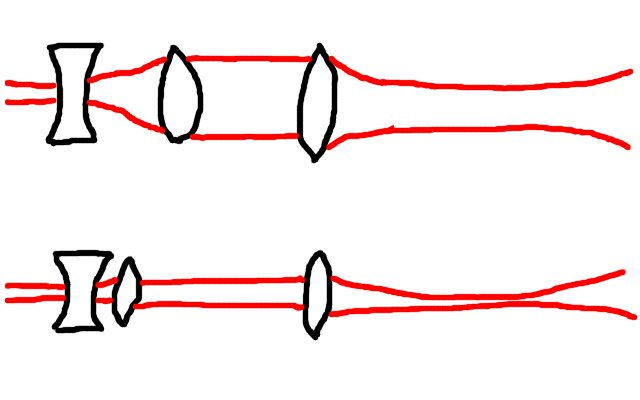
\includegraphics[scale=0.32]{figs/waistcontrol.jpg}
	\caption[Title]{An example setup for controling the beam waist}
	\label{figs/MOT.pdf}
\end{figure}

